\documentclass[12pt]{article}
\usepackage[utf8]{inputenc}
\usepackage{graphicx}
%\usepackage[margin=0.5in]{geometry}
\usepackage{hyperref}
\title{\Huge{Unbabel Java Challenge}}
\author{Tomasz Szypuła}
\date{\today}

\begin{document}
\maketitle
\section{Project Overview and Objectives }
\paragraph{The goal}of the challenge was to write a Java Application meeting the requirements specified in the \href{ https://github.com/Unbabel/java-coding-challenge}{java-coding-challenge}.

 


\section{The Application}
\subsection{How to run the Application}
As mentioned before the application is made using \href{https://openjfx.io/javadoc/11/}{JavaFX}. The application can be deployed as a
\begin{itemize}
\item standalone application
\item standalone self-contained application package
\item web application
\item embedded in a web page
\end{itemize}
For the purpose of this challenge I have deployed my application as a runnable \texttt{.jar} file. In order to execute the \texttt{.jar} file(assuming you are in the directory with the \texttt{.jar} file) one can use the following command: 
\paragraph{}
\texttt{java --module-path \$PATH\_TO\_JAVAFX/javafx-sdk-11.0.2/lib \\--add-modules=javafx.controls,javafx.fxml \\-jar java-coding-challenge.jar \$USERNAME \$API\_KEY}
\paragraph{}
Where 
\begin{itemize}
\item \texttt{\$PATH\_TO\_JAVAFX} is the directory containing the \href{https://openjfx.io/javadoc/11/}{JavaFX} SDK which can be downloaded for example  \href{https://gluonhq.com/products/javafx/}{here}
\item \texttt{\$USERNAME} username to the Unbabel Sandbox API
\item \texttt{\$API\_KEY} api key to the Unbabel Sandbox API
\end{itemize}

\begin{figure}
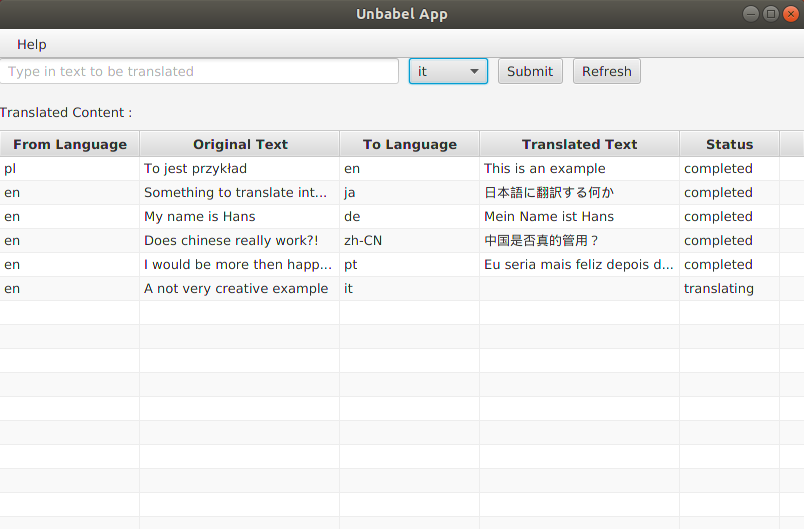
\includegraphics[scale=0.5]{appExample.png}
\end{figure}
\end{document}